\subsection{Relaxationsgleichungen}
\subsubsection{Die allgemeine Relaxationsgleichung}
%
Wird ein System aus seinem Ausgangszustand entfernt und kehrt in diesen zurück, spricht man von Relaxationsprozessen.
Die betrachtete Größe wird hier mit $A$ bezeichnet, wobei $A(t)$ zeitabhängig ist.
Für die zeitliche Änderungsgeschwindigkeit zur Zeit $t$ gilt bei nicht-oszillatorischen Auslenkungen meist folgende Proportionalität
\begin{align}
    \label{eq:proportionalitaet}
    \frac{\diff{A}}{\diff{t}} = c \cdot [A(t) - A(\infty)],
\end{align}
wobei $c$ eine Konstante ist.
Durch Integration und Umformung der Gleichung \eqref{eq:proportionalitaet} folgt die allgemeine Relaxationsgleichung
\begin{align}
    \label{eq:allg_relaxationsglg}
    A(t) = [A(0) - A(\infty)] \cdot \exp{(ct)} + A(\infty),
\end{align}
wobei $c < 0$ gelten muss, damit $A$ beschränkt ist.

\subsubsection{Anwendung auf einen RC-Kreis}
Ein wichtiges Beispiel für nicht-periodische Relaxationsvorgänge ist die Auf- und Entladung (Schalter auf 2 bzw. 1) eines Kondensators über einen Widerstand, 
wie es in Abbildung \ref{fig:auf_und_entladung} zu sehen ist.
Dabei steht $C$ und $Q$ für die Kapazität und Ladung des Kondensators, $U_\text{C}$ für die Spannung am Kondensator und $R$ gibt den Ohmschen Widerstand an.
Die Strömstäke wird mit $I$ bezeichnet, $U_0$ gibt die angeschlossene Gleichspannung beim Aufladen an.
\begin{figure}[H]
    \centering
    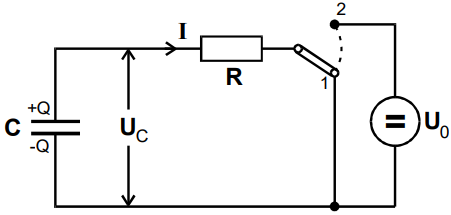
\includegraphics[height = 5cm]{./abbildungen/auf und entladung.png}
    \caption{Schaltkreis zur Auf- und Entladung eines Kondensators \cite{man:v353}.}
    \label{fig:auf_und_entladung}
\end{figure}

\noindent
Für den Entladevorgang eines Kondensators gilt die Randbedingung $Q(\infty) = 0$.
Zusammen mit 
\begin{align}
    U_\text{C} &= \frac{Q}{C}, & I &= \frac{U_\text{C}}{R}, & \diff{Q} &= - I \diff{t}
    \label{eq:gesetze}
\end{align}
ergibt sich somit gemäß Gleichung \eqref{eq:allg_relaxationsglg} die zeitliche Kondensatorladung
\begin{align}
    Q(t) = Q(0) \cdot \exp\left(- \frac{t}{RC}\right)
    \label{eq:entladung}
\end{align}
für den Entladevorgang.

\noindent
Ganz analog folgt für den Aufladevorgang mit den Randbedingungen
\begin{align*}
    Q(0) &= 0, & Q(\infty) &= C U_0 
\end{align*}
die Formel 
\begin{align}
    Q(t) = C U_0 \cdot \left(1-\exp\left(-\frac{t}{RC}\right)\right).
\end{align}
für die Ladung am Kondensator.

\noindent
Sowohl beim Auf- als auch beim Entladevorgang bezeichnet
\begin{align}
    \tau = R C
\end{align}
die sogenannte Zeitkonstante des Relaxationsvorgangs.
Da sich während des Zeitintervalls $\tau$ die Kondensatorladung genau um $1/e$ ändert,
ist $\tau$ somit ein Maß dafür, wie schnell das System gegen den Endzustand $Q(\infty)$ geht.